L'applicazione mobile CAMUS si pone come l'altro elemento fondamentale assieme al server dell'architettura. Ha lo scopo di fornire all'utente finale l'interfaccia per accedere al sistema e semplificare l'utilizzo e l'accesso ai dati. Nel capitolo verrà inizialmente fatta una rapida panoramica per quanto riguarda il cross-platform a livello mobile, in modo da introdurre meglio le tecnologie che sono state utilizzate per implementare l'applicazione. Poi è presente una spiegazione generale delle tecnologie che sono state impiegate nell'applicazione, come React Native e Flux. Successivamente si parlerà di come è stata realizzata l'architettura interna dell'applicazione, partendo dallo schema per definire le pagine e arrivando alla logica di aggiornamento dei dati, seguendo il principio del flusso dati unidirezionale. In seguito verrà definita la struttura del file di mashup proveniente dal server e che è indispensabile per la creazione delle schermate, per poi trattare nello specifico i metodi che occorrono per costruire queste schermate.
Successivamente si tratterà di spiegare il flusso dati all'interno dell'applicazione e poi di come vengono trattate le richieste dati verso il server, con l'utilizzo di GraphQL, per definire le richieste per quanto riguarda il login e di risultati contestuali per l'utente. In conclusione verrà trattato l'argomento riguardante i servizi di supporto.

\section {Architettura dell'applicazione}\label{sec:architettura-applicazione}

\begin{figure}[ht]
	\centering
	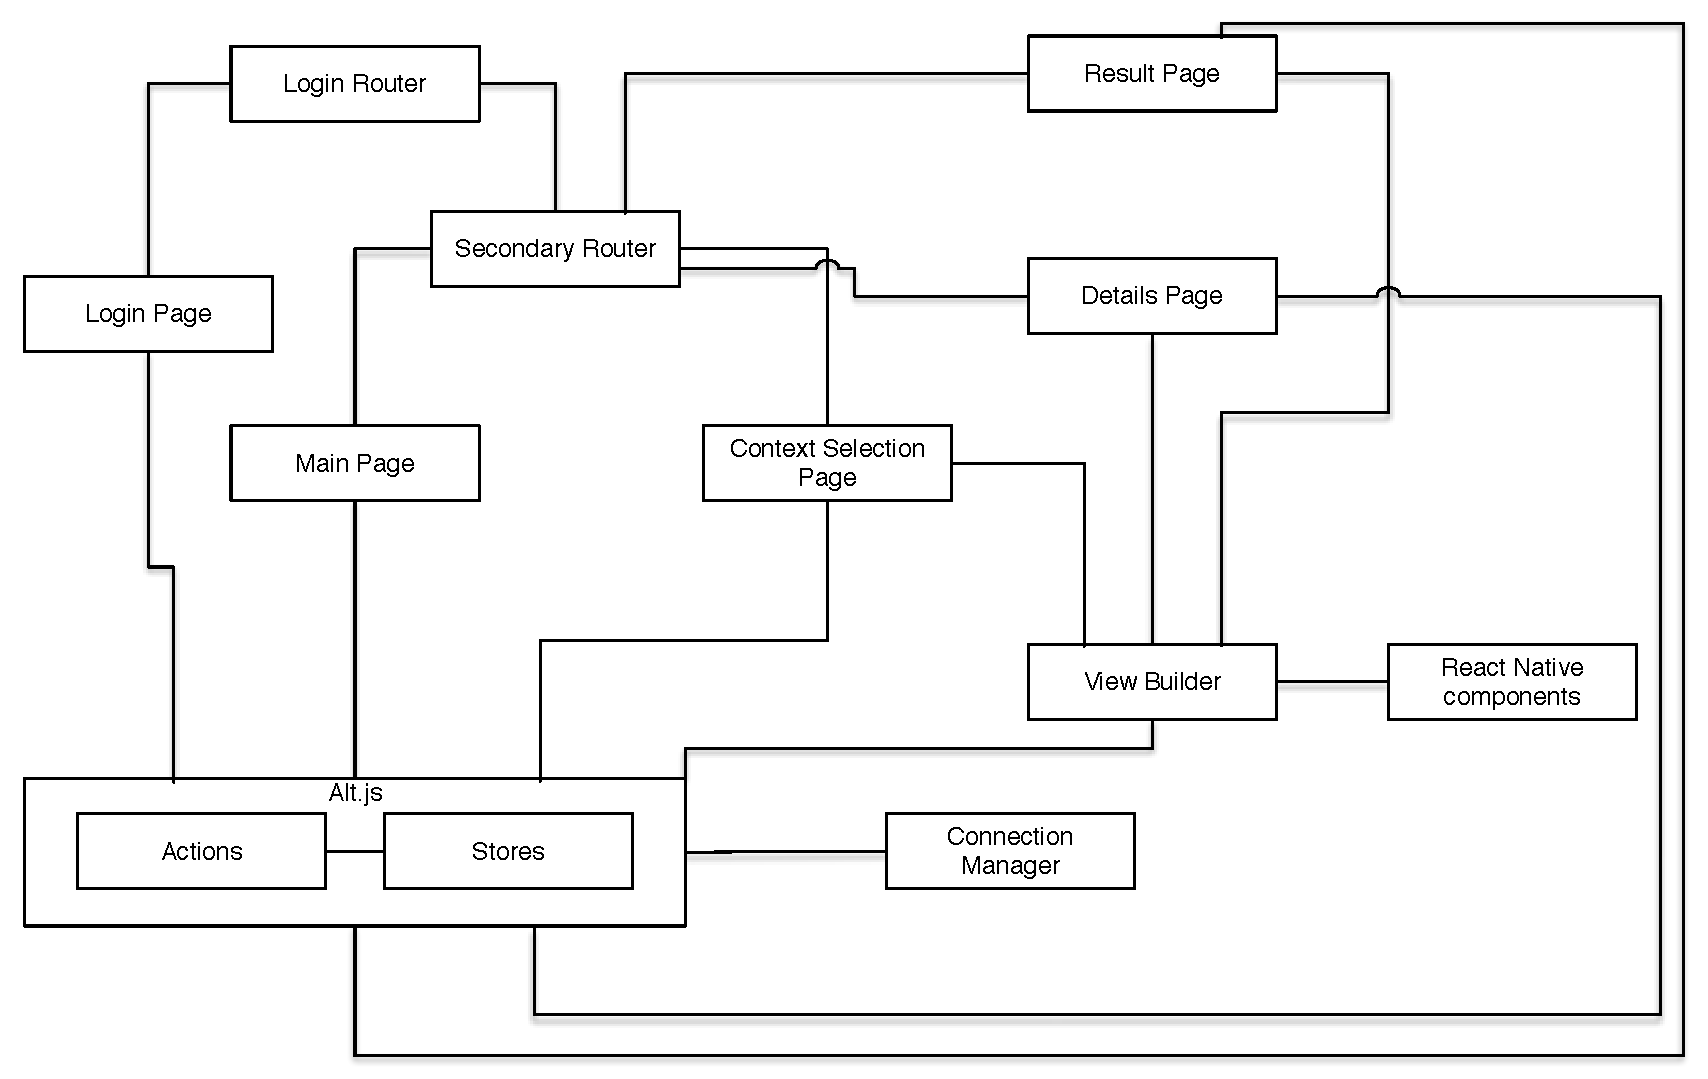
\includegraphics[width=\textwidth]{6-implementazione-app/immagini/app_architecture.pdf}
	\caption{Architetture generale dell'app CAMUS}\label{fig:app-architecture}
\end{figure}

La figura \ref{fig:app-architecture} rappresenta l'architettura dell'applicazione CAMUS. Di seguito sono elencati i componenti principali che definiscono il funzionamento dell'applicazione. 

\subsection{Pagine dell'applicazione}
Essendo un progetto basato su JavaScript per poter controllare le diverse pagine dell'applicazione è necessario utilizzare un router. Si è scelto di sfruttare due router diversi, uno per gestire il login e un altro per la navigazione all'interno dell'applicazione. Il router per il login controlla solamente se l'utente è loggato e ha la funzione di non permettere l'accesso alle pagine che necessitano di autenticazione. Come routes possiede \emph{Login Page} e il secondo router, che racchiude la navigazione effettiva dell'utente autenticato.
\begin{figure}[ht]
	\centering
	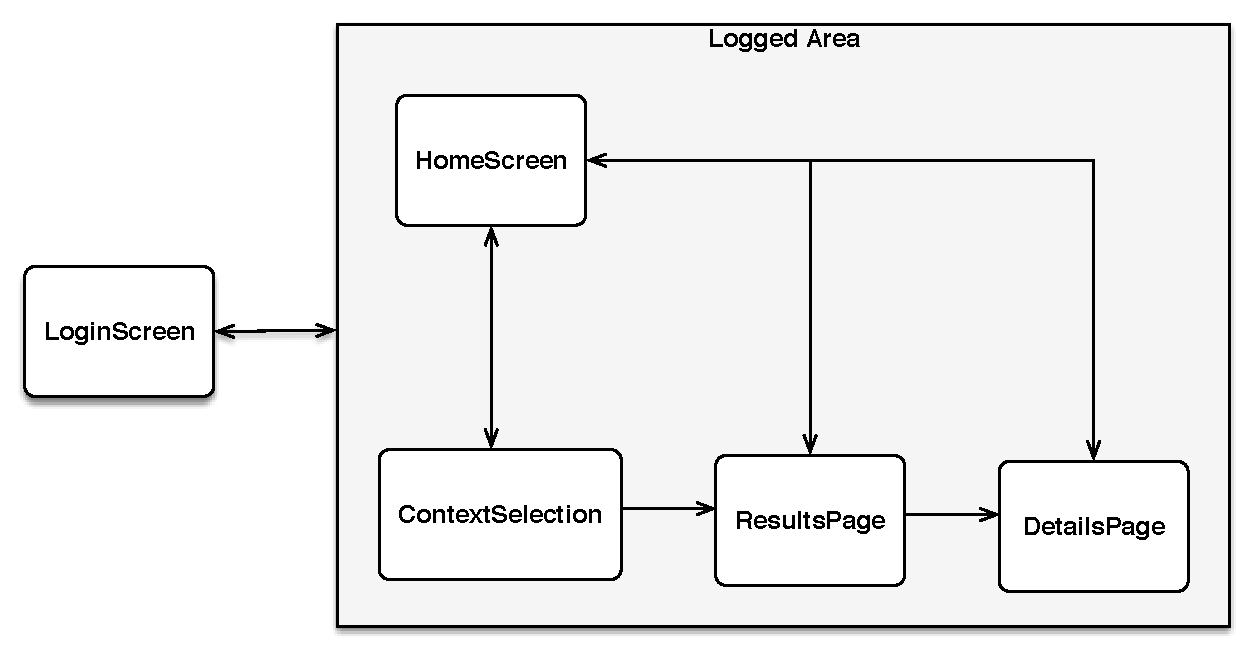
\includegraphics[width=\textwidth]{6-implementazione-app/immagini/screen-schema.pdf}
	\caption{Schema delle pagine}\label{fig:screen-schema}
\end{figure}
Come si può notare nella Figura \ref{fig:screen-schema}, le pagine sono le seguenti:
\begin{itemize}
	\item \textbf{LoginPage} \upe la pagina dove l'utente inserisce le proprie credenziali per accedere al sistema CAMUS e ottenere i parametri per il corretto funzionamento dell'applicazione
	\item \textbf{Logged Area} Si tratta della parte dell'applicazione alla quale l'utente può accedere nel caso in cui sia autenticato e gestisce le pagine di composizione del contesto e di visualizzazione dati:
	\begin{itemize}
		\item \textbf{Main Page} È la pagina principale dell'applicazione e permette all'utente di mostrare tutti le \emph{Interest Topic} associati a lui nel suo CDT. La scelta di quella desiderata permette di accedere alla \emph{Context Selection Page}
		\item \textbf{Context Dimension Page} In questa pagina è chiesto il contesto all'utente mediante un' interfaccia che si adatta alle scelte da lui già eseguite per guidarlo nella definizione del contesto da inviare come richiesta al server. Una volta terminata la scelta viene costruita la query e inviata all'endpoint GraphQL del server CAMUS. 
		\item \textbf{Results Page} Si tratta della pagina che deve mostrare l'intero dataset proveniente dal server e gestisce la paginazione dei risultati, a seconda della posizione del cursore dell'utente nella ListView. 
		\item \textbf{Details Page} In questa pagina vengono visualizzati i dettagli dell'oggetto selezionato e sono gestiti i collegamenti con le applicazioni esterne, per mezzo della libreria di \emph{Linking} di React Native o moduli personalizzati
	\end{itemize}
\end{itemize}

\subsection{Helpers}
Le pagine spiegate nella sezione precedente si servono di alcuni componenti che sono in comune tra tutte le pagine dell'applicazione, che aiutano ad eseguire funzionalità in comune. Di seguito sono elencati i componenti che svolgono questo compito:

\begin{itemize}
	\item \textbf{View Builder} Si tratta del componente che costruisce le view dinamiche partendo dal file di mashup. 
	\item \textbf{Connection Manager} In questo componente vengono gestite tutte le connessioni con l'endpoint GraphQL. Permette di gestire la fase di login e di scambio di dati per scaricare il CDT, gli schemi di mashup e i dati. Per quanto riguarda i dati sono esposti due metodi distinti, il primo per gestire la prima richiesta di nuovi dati, il secondo per le successive, chiedendo una nuova pagina, come spiegato nella sezione \ref{sec:paginazione-app}
	\item \textbf{StyleSheet} Si tratta del foglio di stile nel quale sono impostati tutti i parametri predefiniti per la visualizzazione dei componenti dell'applicazione
\end{itemize}

\subsection{Actions}\label{sec:actions}
Le \emph{Actions} sono i metodi invocati dall'applicazione per modificare lo stato dell'applicazione. Nell'applicazione CAMUS sono utilizzate principalmente in due modi: 
\begin{itemize}
	\item \textbf{Data Fetching} Quando è necessario scaricare gli elementi necessari per il corretto funzionamento dell'applicazione, CDT e mashup, o i dati provenienti dalle richieste, le action hanno lo scopo di modificare lo stato per cambiare la view dell'applicazione a seconda dello stato della richiesta.
	Ad esempio quando si preme il bottone per effettuare una nuova richiesta basata sul contesto, viene invocata un'azione per mantenere lo stato coerente tra più componenti e permettere di mostrare quando ci si trova ancora in fase di caricamento uno Spinner, e una volta che i dati sono arrivati all'interno dell'applicazione mostrarli nella ListView
	\item \textbf{Application State} Lo stato generale dell'applicazione viene salvato utilizzando delle \emph{Action} chiamate dalle interazioni dell'utente con la interfaccia grafica. Ad esempio quando viene composto il contesto per effettuare la query per i risultati le diverse selezioni sono passate tramite le Action nelle Store
\end{itemize}	

Le \emph{Actions} che sono state implementate nell'applicazione sono le seguenti:
\begin{itemize}
	\item \textbf{User Actions} Sono le azioni che servono ad aggiornare i parametri relativi all'utente, come password, email, id del CDT e suo id nel database
	\begin{itemize}
		\item \textbf{Update Email} Metodo per aggiornare l'email dell'utente 
		\item \textbf{Update Password} Metodo per aggiornare la password dell'utente
		\item \textbf{Update Token} Metodo per tenere in memoria il Token della connessione col server per ottenere il CDT
		\item \textbf{Update UserID} Metodo per memorizzare l'id dell'utente del server CAMUS
	\end{itemize}
	\item \textbf{Context Actions} Sono le azioni che gestiscono la selezione del contesto, consentendo di modificare le scelte effettuate dall'utente
	\begin{itemize}
		\item \textbf{Set Transport} Metodo per salvare la tipologia di trasporto da parte dell'utente
		\item \textbf{Set Typology} Metodo per salvare la tipologia nel caso di trasporto non con mezzi propri
		\item \textbf{Add Forbidden} Metodo per aggiungere un parametro in quelli da nascondere all'utente
		\item \textbf{Remove Forbidden} Metodo per rimuovere il parametro selezionato dalla lista di quelli da nascondere all'utente
		\item \textbf{Update Last Context} Metodo per salvare l'ultimo contesto inviato al server nella query per ottenere i risultati richiesti dall'utente, per poterlo riutilizzare nelle richieste per le pagine successive
	\end{itemize}
	\begin{itemize}
		\item \textbf{Update Email} Metodo per aggiornare l'email dell'utente 
		\item \textbf{Update Password} Metodo per aggiornare la password dell'utente
		\item \textbf{Update Token} Metodo per tenere in memoria il Token della connessione col server per ottenere il CDT
		\item \textbf{Update UserID} Metodo per memorizzare l'id dell'utente del server CAMUS
	\end{itemize}
	\item \textbf{View Actions} Sono le azioni relative alla gestione dei mashup, ma non dello stato della navigazione, per le quali è utilizzato un componente aggiuntivo sempre basato su Flux (React Native Router Flux)
	\begin{itemize}
		\item \textbf{Set Views} Metodo per salvare il file con le view provenienti dal server 
		\item \textbf{Select Interest Topic} Metodo per salvare l'\emph{Interest Topic} corrente selezionato da parte dell'utente
	\end{itemize}
	\item \textbf{Data Actions} Trattano della gestione del CDT e dei risultati ottenuti dal server
	\begin{itemize}
		\item \textbf{Update Results} Metodo per aggiornare i dati dei risultati provenienti dalla query basata sul contesto
		\item \textbf{Results Failed} Metodo per inviare il messaggio di errore proveniente dalla richiesta
		\item \textbf{Update Full CDT} Metodo per aggiornare il CDT associato all'utente
		\item \textbf{Update Id CDT} Metodo per salvare soltanto l'ID del CDT
		\item \textbf{Update UserID} Metodo per memorizzare l'id dell'utente del server CAMUS
	\end{itemize}
\end{itemize}


\subsection{Stores}\label{sec:action-store}
Le \emph{stores} sono il modulo dove lo stato dell'applicazione viene salvato e forniscono alle view nuovi dati ogni volta che sono aggiornate. 
Per ogni interazione sui dati dell'applicazione che necessitano di rimanere persistenti, viene invocata una action dal componente e dalla view che si propaga prima nelle store, e successivamente aggiorna nuovamente la view.
Si è scelto di suddividere le \emph{Store} per tipologia di operazione e dato trattata:
\begin{itemize}
	\item  \textbf{User Store} Nella \emph{User Store} sono memorizzati tutti i dati relativi all'utente. In particolare viene memorizzato l'Id dell'utente nel database del server e l'Id del CDT a lui associato, che serviranno per poter effettuare le query GraphQL per ottenere i dati
	\item \textbf{Context Store} Nel \emph{Context Store} vengono gestiti i dati che riguardano i dati di contesto, come le coordinate geografiche e le scelte delle tipologie di trasporto pubblico, in modo da essere riutilizzate. Per quanto riguarda le richieste di dati, una volta che il contesto viene composto per effettuare la prima query, questo payload viene salvato qui e poi riutilizzato nelle query dei risultati successivi
	\item \textbf{View Store} In questa store sono memorizzati tutti i dati relativi alle view. Qui viene salvato lo schema di mashup e l'\emph{Interest Topic} corrente
	\item \textbf{Data Store} Si tratta della store più complessa perchè deve gestire in modo dinamico diverse tipologie di dato. Quando viene ricevuto il CDT vengono scanditi gli \emph{interest topic} creato un oggetto nel campo \emph{results} che è composto da un array di tanti oggetti definiti da due campi:
	\begin{enumerate}
		\item \textbf{Results} Rappresenta i risultati ricevuti per quell'\emph{interest topic} dal server, con i risultati provenienti dai servizi primari e i collegamenti per i servizi di supporto
		\item \textbf{Topic} Rappresenta l'\emph{Interest topic} associato ai risultati ricevuti dal server
	\end{enumerate}
	Questa operazione è necessaria per poter gestire il fatto di avere comunque dei dati in memoria in condizioni di assenza di rete, anche per tipi diversi di risultati provenienti dal server e per essere in grado di gestire una cardinalità variabile di tipologie di dati. Nel Listato \ref{lst:store-two-topics} è mostrato come viene rappresentato lo stato nel caso in cui l'utente abbia a disposizione due \emph{Interest Topic} e la suddivisione dei risultati per quanto riguarda le due tipologie, in questo caso \emph{Restaurants} ed \emph{Event}. Si noti che oltre ai risultati sono salvati anche i parametri con lo stato della paginazione, per lasciare la possibilità di riprendere la visione di nuovi risultati.
	
\end{itemize}

\begin{lstlisting}[backgroundcolor = \color{lightgray},
								caption = Esempio Data Store Mashup,
								label = lst:store-two-topics]
				results: 
				   [ { topic: 'Restaurant',
				       results: 
				        { primaryResults: 
				           {data: 
			                   { title: 'Peck',
			                     address: 'Via Spadari, 9, Milano',
			                     longitude: '9.187005400000002',
			                     latitude: '45.4635272',
			                     email: null,
			                     meta: { rank: 1, name: [ 'GooglePlaces' ] } } ,
			                   { title: 'Ristorante Al Mercante',
			                     address: 'Piazza dei Mercanti, 17, Milano',
			                     longitude: '9.1872837',
			                     latitude: '45.4647966',
			                     email: null,
			                     meta: { rank: 1, name: [ 'GooglePlaces' ] } } ,
			                   { title: 'Ristorante Pizzeria Maruzzella',
			                     address: 'Piazza Guglielmo Oberdan, 3, Milano',
			                     longitude: '9.2048763',
			                     latitude: '45.4752701',
			                     email: null,
			                     meta: { rank: 1, name: [ 'GooglePlaces' ] } } ,
			                   { title: 'Ristorante Cracco',
			                     address: 'Via Victor Hugo, 4, Milano',
			                     longitude: '9.1871136',
			                     latitude: '45.4639508',
			                     email: null,
			                     meta: { rank: 1, name: [ 'GooglePlaces' ] } } ,
			                   { title: 'ristorante vietnamonamour',
			                     address: 'Via Alessandro Pestalozza, 7, Milano',
			                     longitude: '9.2226117',
			                     latitude: '45.48151049999999',
			                     email: null,
			                     meta: { rank: 1, name: [ 'GooglePlaces' ] } } ,
				             pageInfo: { endCursor: 'YXJyYXljb25uZWN0aW9uOjg=', hasNextPage: true } },
				          supportResults: { data: [] } } },
				     { topic: 'Event',
				       results: 
				        { primaryResults: 
				           data:
			                   { title: 'Gemitaiz',
			                     address: 'Via Valtellina 21',
			                     latitude: '45.4941542',
			                     longitude: '9.1827734',
			                     meta: { rank: 1, name: [ 'eventful' ] } } ,
			                   { title: 'Closer #7 /// Violet Poison - Fedex - Rorschack at Masada',
			                     address: 'Viale Carlo Espinasse, 41',
			                     latitude: '45.4667',
			                     longitude: '9.2',
			                     meta: { rank: 1, name: [ 'eventful' ] } } ,
			                   { title: 'Congrès de l\'Impression d\'Europe du Sud - Southern European Print Congress 2016',
			                     address: 'ITALY',
			                     latitude: '45.4667',
			                     longitude: '9.2',
			                     meta: { rank: 1, name: [ 'eventful' ] } } ,
			                   { title: 'THE DICTATORS NYC',
			                     address: 'Via Circonvallazione Idroscalo, 41',
			                     latitude: '45.4667',
			                     longitude: '9.2',
			                     meta: { rank: 1, name: [ 'eventful' ] } } ,
			                   { title: 'STEVE\'N\'SEAGULLS',
			                     address: 'Via Circonvallazione Idroscalo, 41',
			                     latitude: '45.4667',
			                     longitude: '9.2',
			                     meta: { rank: 1, name: [ 'eventful' ] } } ,
				             pageInfo: { endCursor: 'YXJyYXljb25uZWN0aW9uOjg=', hasNextPage: true } },
				          supportResults: { data: [] } } } ],
				}

\end{lstlisting}

\section{Struttura dello schema di mashup}

Per poter permettere una dinamicità nell'applicazione si è scelto di utilizzare uno schema di mashup molto semplice e allo stesso tempo sufficientemente potente. Si è scelto di utilizzare uno schema di tipo JSON in modo da essere facilmente sfruttato all'interno del motore JavaScript di React Native. 
Nel caso di CAMUS l'oggetto che è presente nelle view considera due tipologie di view diverse: la \emph{list} e la \emph{details}. Nella tipologia \emph{list} sono definite le view che definiscono il singolo item della ListView e generalmente si compone di una quantità non eccessiva di componenti
Nella tipologia \emph{details} sono disponibili tutti i dettagli dell'item selezionato e sono definiti tutti i termini necessari a identificare l'elemento per l'utente.
Considerando l'esempio dei ristoranti, per la lista sono associati i termini che servono per identificare l'oggetto, come il nome e l'indirizzo. Se poi l'utente vuole vedere la mappa dove si trova e visualizzare gli estremi per contattare il ristorante per prenotare, deve aprire la pagina dei dettagli, dove prendendo i termini dal file di mashup, sono visualizzati tutti i dettagli necessari per l'utente. Inoltre è specificata la tipologia dell'elemento da visualizzare, in modo da permettere all'app di utilizzare le librerie di collegamento con le applicazioni specifiche del sistema operativo mobile.

Nel Listato \ref{lst:mashup-schema} sottostante è espresso un frammento del file JSON di mashup della pagina di dettaglio:
\begin{lstlisting}[backgroundcolor = \color{lightgray},
								caption = Esempio Schema Mashup,
								label = lst:mashup-schema]
	{	
		details: 
			[ 
				{ 
					topics:	
						[ 
							'Restaurant',
							'Event' 
						],
					contents: 
						[ 
							{ 
								type: 'text', 
								contents: 'title' 
							},
							{ 
								type: 'text', 
								contents: 'address'
							},
							{ 
								type: 'map', 
								contents: [ 'latitude', 'longitude' ] 
							},
							{ 
								type: 'phoneNumber', 
								contents: 'telephone' 
							},
							{ 
								type: 'website', 
								contents: 'website' 
							},
							{ 
								type: 'email',
								contents: 'email' 
							},
							{ 
								type: 'support', 
								contents: 'Transport' 
							}
						] 
					}
				]	
		}
	
\end{lstlisting}

Di seguito invece sono elencate le diverse tipologie di dato che compongono l'oggetto che rappresenta i file di \emph{mashup}:
\begin{itemize}
	\item \textbf{Type} Il termine \emph{type} indica il tipo dell'elemento da visualizzare nella view. È associato ad un componente React Native, che verrà richiamato quando verrà costruita l'interfaccia grafica
	\item \textbf{Topic} Si tratta di un array di stringhe e questo elemento indica tutte le aree di interesse che sono associate allo schema in questione. Si è scelto di utilizzare una struttura basata su tag, cioè quando l'applicazione deve accedere alla struttura del mashup viene scelto lo schema nel quale è taggato in questo campo il valore dell'\emph{Interest Topic} attualmente selezionata dall'utente
	\item \textbf{Contents} Indicano tutti i contenuti di tipo dato o figli di un altro elemento \emph{content}. Se nell'oggetto padre è indicato un oggetto \emph{type}, gli elementi in \emph{contents} rappresentano i termini da richiedere nella query GraphQL per ricevere i dati dal server. In caso contrario questo campo indica che in \emph{contents} è presente un nuovo livello di annidamento. Ci possono essere tanti annidamenti, fino a quando non si arriva ad avere un oggetto che possiede il campo \emph{type}
	\item \textbf{Style} Nel caso in cui a livello di design del mashup si voglia definire uno stile personalizzato diverso da quelli di default, in questo campo si può definire un oggetto di tipo Flexbox, interpretabile da React Native, che viene applicato all'elemento corrente. 
\end{itemize}

\section{Rendering delle view}\label{sec:rendering-view}

Si tratta della funzionalità più delicata da progettare all'interno dell'applicazione, perché non è così semplice pensare di generare in modo dinamico delle pagine con così tanta mutabilità a partire da un documento strutturato delle interfacce visuali dinamiche.
Mentre in codice nativo questo problema può presentare delle difficoltà a livello implementativo, l'utilizzo da parte di React di un Virtual DOM simile al linguaggio HTML offre il vantaggio di poter generare molto rapidamente una traduzione dal file di mashup ad un modello interpretabile dal motore di rendering dell'app.
Per questo motivo è stato creato un componente apposito, il View Render, che, dato un oggetto contenente il mashup, riesce a fare l'associazione dei contenuti semantici all'interno di questo, con i componenti presenti nell'applicazione, generando un nuovo oggetto strutturato pronto per essere tradotto in visualizzazione dall'oggetto padre della pagina.
Sono presenti all'interno due tipologie di rendering: il rendering del contesto e il rendering dei risultati.

\subsection{Contesto} 
Nel caso del rendering della pagina di contesto non si ritiene necessario l'utilizzo di un mashup esterno, in quanto tutte le informazioni presenti all'interno del CDT sono sufficienti a definire in modo corretto la sua visualizzazione e la sua compilazione da parte dell'utente.
	Per ogni oggetto facente parte del CDT viene eseguita un'associazione a componenti già esistenti della view e che non sono modificabili dall'esterno.
	\begin{itemize}
		\item \textbf{Interest Topic} Per quanto riguarda le \emph{Interest Topic} hanno bisogno di essere selezionate nella pagina iniziale appena dopo il login, e vengono caricate in una lista di bottoni con due elementi per riga, con un'icona rappresentativa. I bottoni e le icone sono predefinite nell'applicazione e necessitano soltanto di una associazione nome elemento dal campo \emph{Interest Topic} all'interno del CDT. Questa funzione molto semplice viene eseguita direttamente all'interno della pagina principale, senza la necessità di utilizzare il View Render
		\item \textbf{Altri elementi} Gli altri elementi del contesto sono processati all'interno del componente View Builder. Con una funzione ricorsiva viene scandito l'intero CDT ricevuto dal server con i campi da modificare e in base ai contenuti viene costruito l'elemento della view, a seconda della tipologia. Ad esempio se per un campo è richiesto l'inserimento di un numero verrà mostrato un TextInput che permette il completamento solo con numeri, mentre se ho a disposizione una scelta tra più elementi verrà mostrata una lista selezionabile.
		Assume una grande importanza anche la gestione delle esclusioni tra le operazioni. Se viene selezionato \virgolette{With Car}, non è corretto mostrare le possibili tipologie di trasporto pubblico, perché si conosce già a priori che l'utente non selezionerà mai nello stesso momento come mezzo di trasporto l'automobile e il bus. Per questo scopo all'interno della \emph{Context Store} vengono gestiti con una struttura dati ad Array i nodi che non devono essere mostrati e questa variabile viene aggiornata con le selezioni che sono state fatte nell'interfaccia utente all'interno della pagina di contesto
	\end{itemize}
	
\subsection{Risultati}\label{sec:view-risultati}
Per quanto concerne i risultati ottenuti dalle query dal server GraphQL entrano in gioco in maniera preponderante gli schemi di mashup. Per i motivi spiegati in \ref{sec:mashup-design}, la risoluzione del problema necessita di un funzionamento più complesso rispetto alla visualizzazione del contesto. La funzione di rendering per quanto riguarda i risultati è la medesima sia per la lista che per i dettagli, quello che cambia è il contenitore del componente View Builder: per la lista è un figlio nel metodo di \emph{renderItem()} della ListView, mentre per i dettagli definisce l'intera pagina.
	Al componente View Render sono necessari due oggetti: il file di mashup e i dati del singolo risultato.
	Si suppone che nel file di mashup gli elementi siano già stati generati in ordine di visualizzazione, perché nella funzione di costruzione non è possibile modificarlo. Tuttavia, è possibile modificare lo stile più esterno del componente risultante per cambiare il layout dei figli del \emph{View Builder}. Per prima cosa il \emph{View Builder} deve scegliere le view associate all'\emph{Interest Topic} facendo una ricerca della prima vista che contiene il valore corrente dell'\emph{Interest Topic} e passare questo oggetto alla funzione di rendering. A questo punto si è pronti per costruire la view del componente: viene scandito ogni elemento del file di mashup e si associa il valore dato dal termine dell'oggetto del risultato e viene ritornato il componente pronto per essere elaborato per la visualizzazione. Nel caso in cui non fosse presente un valore per il termine desiderato ovviamente non viene renderizzato nessun elemento, ritornando una \emph{View} base vuota, che non ha nessuna incidenza sulla grafica avendo dimensione nulla. Nel caso in cui esista un oggetto di tipo \emph{style}, esso ha la priorità rispetto a quello presente nel foglio di stile predefinito dell'applicazione. Per il momento sono disponibili queste tipologie di componenti specificabili nel campo \emph{type} dell'oggetto di mashup e che sono pienamente supportati:
	\begin{itemize}
		\item \textbf{Text} è il componente di testo base, per la sua differenziazione si utilizzano attributi diversi nel foglio di stile in comune per tutta l'applicazione o le specifiche presenti nell'attributo \emph{style} del mashup
		\item \textbf{Map} è il componente che renderizza le mappe. Presenta due implementazioni differenti per quanto riguarda iOS e Android, poiché come mappe di sistema hanno due applicazioni differenti. Per quanto iOS sono presenti le mappe di Apple che sono già integrate nel componente \emph{MapView} di React Native, mentre per Android sono presenti le mappe di Google Maps, per le quali è stato utilizzato un componente esterno, il cui funzionamento è molto simile alla MapView
		\item \textbf{Website} Permette di gestire il sito web dell'elemento, contenendo anche la funzione per invocare il browser di sistema e visualizzarlo
		\item \textbf{Email} Permette di visualizzare l'indirizzo di email dell'elemento e selezionando l'icona di invio email l'utente viene reindirizzato all'applicazione o alla scelta di un'applicazione per inviare un messaggio email all'indirizzo specificato
		\item \textbf{Phone} Questo componente gestisce il numero di telefono dell'elemento, con la possibilità di inviare un messaggio al numero o di effettuare una telefonata, sempre utilizzando le applicazioni predefinite del dispositivo mobile
		\item \textbf{Support} Si tratta del componente che gestisce i servizi di supporto con i collegamenti alle applicazioni esterne, verrà spiegato nei dettagli nella Sezione \ref{sec:servizi-supporto-app}
	\end{itemize}

\subsection{Gestione degli stili}

Per quanto riguarda la gestione degli stili si è scelto di adottare una soluzione molto semplice, ma allo stesso tempo molto efficace. Si è partiti dalla condizione che React Native utilizza come gestione dello stile Flexbox\footnote{Flexbox su W3Schools: \url{http://www.w3schools.com/css/css3_flexbox.asp}}, che è una modalità di stile CSS che è ottimizzata per la gestione degli elementi per quanto riguarda le differenti dimensioni degli schermi. Il linguaggio utilizzato risulta essere molto simile a JSON e quindi è facilmente integrabile in JavaScript. L'elemento che gestisce gli attributi grafici è lo \emph{StyleSheet} che espone l'oggetto \emph{styles} e gli attributi \emph{PRIMARY\_COLOR} e \emph{SECODARY\_COLOR}.
Nell'oggetto \emph{styles} sono impostati tutti gli stili di ogni componente grafico dell'applicazione, che vengono richiamati nella fase di costruzione delle view. In questo modo ogni modifica all'interno dell'oggetto si ripercuote in tutta l'applicazione.
I due attributi per la gestione dei colori sono risultati indispensabili in particolare per alcuni componenti, come la \emph{StatusBar} di Android, hanno come elemento impostabile solo il colore e non lo stile completo. Ovviamente la modifica all'interno dello \emph{StyleSheet} dei parametri di colore è necessaria solo in un punto del codice, in modo da propagarsi in modo coerente per l'intera applicazione.
Nel Listato \ref{lst:stylesheet} è mostrato un frammento del foglio di stile utilizzato nell'applicazione. Si noti come i parametri che definiscono ogni singolo elemento sono abbastanza autoesplicativi, fornendo allo sviluppatore una maggiore semplicità di programmazione. Diversi parametri sono stati ripetuti, per permettere la visualizzazione del componente in modo ottimale sia in Android che in iOS.

\begin{lstlisting}[backgroundcolor = \color{lightgray},
								caption = Frammento Foglio di Stile,
								label = lst:stylesheet]
	var styles = StyleSheet.create({
	    container: {
	        flex: 1,
	        backgroundColor: 'white',
	        marginTop: 20
	    },
	    iosContainer: {
	        backgroundColor: 'white',
	        marginTop: 70
	    },
	    iosStatusBar:{
	        color: 'black'
	    },
	    buttonMaterial: {
	        height: 36,
	        backgroundColor: primary_color,
	        borderColor: primary_color,
	        borderWidth: 1,
	        borderRadius: 8,
	        marginBottom: 10,
	        alignSelf: 'stretch',
	        justifyContent: 'center'
	
	    }
	    //altri elementi di stile
	 })   
\end{lstlisting}
 

\section{Flusso di esecuzione}

In questa sezione si vuole affrontare il flusso dei dati all'interno dell'applicazione, partendo dal login da parte dell'utente, fino alla selezione di un elemento dalla lista dei risultati.
\begin{figure}[ht]
	\centering
	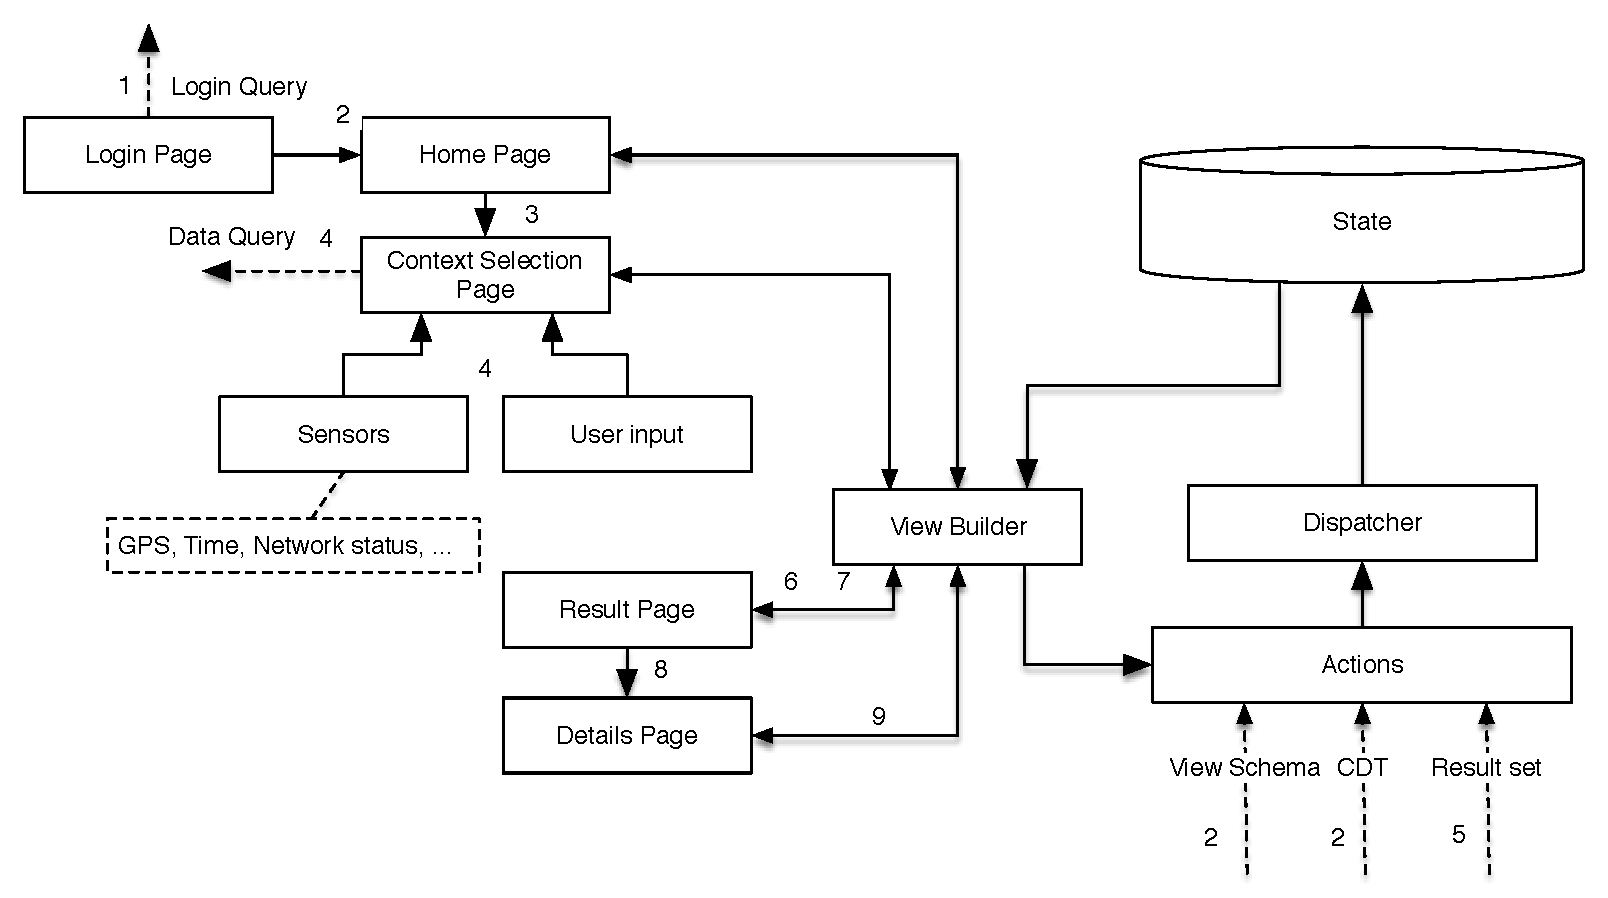
\includegraphics[width=\textwidth]{6-implementazione-app/immagini/app_dataflow.pdf}
	\caption{Flusso dei dati dell'app Flux}\label{fig:app-dataflow}
\end{figure}
Nella Figura \ref{fig:app-dataflow} è rappresentato tutto il flusso dei dati all'interno dell'applicazione e di seguito vengono esposti i passaggi principali:
\begin{enumerate}
	\item La prima schermata che appare nell'applicazione è quella di login; qui l'utente inserisce le proprie credenziali e viene effettuata la richiesta GraphQL di login come definito in \ref{sec:login-endpoint}
	\item Vengono ricevuti il CDT e i mashup dal server e quindi l'applicazione possiede tutto ciò che è necessario a caricare l'interfaccia grafica. Nel frattempo il router mostra la pagina iniziale dell'applicazione
	\item L'utente seleziona l'\emph{Interest Topic} desiderato e viene reindirizzato alla pagina di selezione del contesto, dove vengono mostrati i campi che devono essere compilati dall'utente
	\item Dopo aver definito i parametri del contesto desiderati, l'utente preme sul tasto per effettuare la richiesta al server: l'applicazione recupera i dati inseriti dall'utente e allo stesso tempo i dati di posizione provenienti dai sensori del dispositivo mobile
	\item I dati di contesto sono composti assieme ai dati provenienti dai mashup per costruire la query GraphQL, come spiegato nella sezione \ref{sec:data-query}
	\item Il router dell'applicazione mostra all'utente la pagina dei risultati, la quale fino a quando non arriva una risposta dal server continua a mostrare un'interfaccia di caricamento
	\item I risultati vengono processati insieme ai file di mashup per mostrare i dati nella pagina che mostra la lista di risultati
	\item L'utente scorre il result set ottenuto fino a quando non sceglie un elemento per visualizzarne i dettagli
	\item L'applicazione carica la pagina con i dettagli, dove gli vengono passati i dati completi dell'elemento selezionato e visualizzati nella pagina
\end{enumerate}

\section{Query GraphQL}\label{sec:utilizzo-dati-app}

I dati nell'intero sistema CAMUS assumono un ruolo fondamentale. In questa sezione si vuole affrontare la gestione dei dati all'interno dell'applicazione, partendo dagli algoritmi per costruire le query GraphQL, per poi parlare dell'utilizzo dei dati all'interno dell'applicazione, con la gestione della paginazione dei risultati.
Tutto lo scambio di dati tra l'applicazione e il server viene svolto utilizzando query GraphQL, come spiegato nella Sezione \ref{sec:graphql-introduzione}. Per implementare il modulo di gestione delle connessioni si è scelto di utilizzare \emph{Lokka} \footnote{Github Lokka: \url{https://github.com/kadirahq/lokka}}, un client di GraphQL che permette di gestire le query come se fossero normali \emph{fetch()} di JavaScript e lasciare una configurazione più libera e adattabile alle esigenze del sistema. Questo permette di sfruttare in modo molto aderente alle specifiche il paradigma Flux, salvando la maggior parte del contenuto della risposta nella \emph{Data Store}, con le modalità esposte nella Sezione \ref{sec:action-store} e rendendolo quindi disponibile per tutti i singoli componenti dell'applicazione. Di seguito sono spiegate le due tipologie principali di query gestite con GraphQL, che sono le query di login e le query per accedere ai dati.

\subsection{Login Query}
Le query per gestire il meccanismo di login sono molto semplici. Sono basate sui dati inseriti dall'utente quando si trova nella \emph{Login Page} e sulle risposte intermedie fornite dal server. Queste query servono per ottenere l'id dell'utente, l'id del CDT a lui associato e lo schema dei mashup con le definizioni delle sue view.
I dati necessari per la costruzione della query sono l'indirizzo email e la password, che sono inseriti dall'utente nella prima pagina che gli viene mostrata. A questo punto questi dati sono salvati nella \emph{User Store} e sono tenuti nello stato dell'applicazione, nel caso in cui fosse necessario effettuare una nuova richiesta senza richiederli nuovamente all'utente. Nel caso in cui l'indirizzo email e/o la password sono errati, viene notificato un errore, mentre se uno dei due campi è mancante vengono richiesti nuovamente senza inviare nessuna richiesta, dato che ovviamente la risposta sarebbe negativa.
In caso di risposta affermativa da parte del server vengono restituiti all'utente il proprio id e un token, che viene generato per ogni nuovo login al server. Questo token e l'id sono salvati sempre nella \emph{User Store}, e successivamente inviati al server con la query \emph{getIdCdt()} per ottenere il CDT completo per poter costruire il contesto da mostrare all'utente e l'id del CDT che funge da token assieme all'id dell'utente per effettuare le query per ottenere i dati.
Utilizzando un esempio pratico, dopo che l'utente Mario Rossi ha inserito le proprie credenziali di accesso, cioè indirizzo email e password, vengono restituiti questi dati (Listato \ref{lst:esempio-login-app}): 

\begin{lstlisting}[backgroundcolor = \color{lightgray},
							caption = Esempio di risposta alla query di login,
							label = lst:esempio-login-app]
			{
			  "data": {
			    "login": {
			      "id": "56e69f1085ef170300a7b402",
			      "name": "Mario",
			      "surname": "Rossi",
			      "token": "b6aa96da4c78e6e94468ffa25868867d"
			    }
			  }
			}
\end{lstlisting}

I dati all'interno dei campi \emph{id} e \emph{token} sono inviati al server per ottenere il CDT associato all'utente, ottenendolo come di seguito (Listato \ref{lst:esempio-getcdt-app})


\begin{lstlisting}[caption = Esempio di risposta alla query di login,
							backgroundcolor = \color{lightgray},
							label = lst:esempio-getcdt-app]
			{
			  "data": {
			    "getPersonalData": {
			      "idCdt": "56e69f1085ef170300a7b403",
			      "context": [
			        {
			          "name": "InterestTopic",
			          "values": [
			            "Restaurant",
			            "Event"
			          ],
			          "parameters": [],
			          "parents": []
			        },
			        {
			          "name": "Location",
			          "values": [],
			          "parameters": [
			            {
			              "name": "CityCoord",
			              "type": null,
			              "enum": [],
			              "fields": [
			                {
			                  "name": "Latitude"
			                },
			                {
			                  "name": "Longitude"
			                }
			              ]
			            }
			          ],
			          "parents": []
			        },
			        {
			          "name": "Transport",
			          "values": [
			            "PublicTransport",
			            "WithCar"
			          ],
			          "parameters": [],
			          "parents": []
			        },
			        {
			          "name": "Typology",
			          "values": [
			            "Bus",
			            "Train",
			            "Taxi",
			            "CarSharing",
			            "WithDriver"
			          ],
			          "parameters": [],
			          "parents": [
			            "PublicTransport"
			          ]
			        }
			      ],
			      "defaultValues": []
			    }
			  }
			}
\end{lstlisting}

\subsection{Data Query} \label{sec:data-query}
Le query per gestire i dati necessitano di tutta una serie di operazioni preliminari, perché sono presenti diversi parametri da ricavare per poter formare una richiesta GraphQL per CAMUS. Oltre alla definizione spiegata nella Sezione \ref{sec:endpoint-graphql}, di seguito è spiegata la modalità di costruzione dei parametri che sono necessari alla costruzione della query utilizzando il metodo \emph{client.query()} di \emph{Lokka}:
\begin{itemize}
	\item \textbf{UserId} Si tratta dell'id dell'utente nel database del server. Esso viene ricavato immediatamente alla prima query del processo di login ed è necessario per una questione di sicurezza, in combinazione con l'id del CDT
	\item \textbf{IdCdt} Rappresenta l'id del CDT. Come spiegato nelle sezioni precedenti questo identificativo rappresenta un id personalizzato che viene associato al singolo utente
	\item \textbf{Context} \upe l'oggetto che rappresenta il contesto attuale nel quale si trova l'utente. Quando l'utente ha terminato la compilazione del contesto nella \emph{Context Selection Page} i parametri e i valori sono registrati nella Context Store, ma per essere interpretati dal server necessitano una conversione in un oggetto ben definito. Il problema di una query GraphQL è che l'oggetto in questione deve essere ulteriormente convertito in una stringa unica per poi venire collocato come payload nella POST/HTTP. Per svolgere questo compito viene utilizzata una funzione personalizzata che permette di mantenere inalterata la chiave degli oggetti JavaScript e come output una stringa. Per poter convertire anche gli oggetti che sono innestati ad un livello superiore viene utilizzata una ricorsione che richiama la prima funzione
	\item \textbf{Support} Rappresenta la tipologia di servizi di supporto che l'utente richiede per integrare al meglio i dati che gli necessitano, ad esempio nella demo di CAMUS si utilizzano i servizi di tipo \virgolette{Transport}
	\item \textbf{PrimaryResults} Rappresentano i dati provenienti dai servizi invocati dal server per costruire l'insieme dei risultati per l'utente. GraphQL, come già espresso in precedenza, permette di eseguire delle richieste di dati altamente personalizzate, permettendo di richiedere la minima quantità di dati indispensabile per l'utilizzo da parte dell'utente. Per poter svolgere questo si è scelto di utilizzare i termini semantici dei mashup in particolare della tipologia \emph{details}, perché si suppone che nel caso della lista si abbia un sottoinsieme di termini semantici. Come per quanto riguarda la funzione di costruzione della view espressa nella Sezione \ref{sec:rendering-view}, anche in questo caso è necessario prendere i mashup associati all'\emph{Interest topic} e poi selezionare solamente i termini (Listato \ref{lst:esempio-data-mashup}). A questo punto sono posizionati in una string di termini che verranno inviati al server (Listato \ref{lst:esempio-primary-app})
	\item \textbf{SupportResults} Lo stesso meccanismo utilizzato per i \emph{PrimaryResults} è riproposto anche per i risultati di supporto. Invece di recuperare i mashup dalle \emph{Store}, viene riproposta la stessa definizione per ogni query, perché i servizi di supporto sono definiti sempre nello stesso modo con i campi \emph{category}, \emph{service} e \emph{url}
\end{itemize}

\begin{center}
	\hspace*{-1.5cm}
	\begin{minipage}[t]{0.63\textwidth}
		\begin{lstlisting}[caption=Mashup di partenza, label=lst:esempio-data-mashup]
{	
details: 
[ 
	{ 
		topics:	
			[ 
				'Restaurant',
				'Event' 
			],
		contents: 
			[ 
				{ 
					type: 'text', 
					contents: 'title' 
				},
				{ 
					type: 'text', 
					contents: 'address'
				},
				{ 
					type: 'map', 
					contents: [ 'latitude', 'longitude' ] 
				},
				{ 
					type: 'phoneNumber', 
					contents: 'telephone' 
				},
				{ 
					type: 'website', 
					contents: 'website' 
				},
				{ 
					type: 'email',
					contents: 'email' 
				},
				{ 
					type: 'support', 
					contents: 'Transport' 
				}
			] 
		}
	]	
}
		\end{lstlisting}
	\end{minipage}%
	\begin{minipage}[t]{0.63\textwidth}
		\begin{lstlisting}[caption=Definizione oggetto GraphQL per risultati primari, label=lst:esempio-primary-app,style=json]
				!primaryResults! {
					!data! {
						!title!
						!address!
						!latitude!
						!longitude!
						!meta! {
							!name!
							!rank!
						}
					}
				}
		\end{lstlisting}
	\end{minipage}	
\end{center}

Nel listato \ref{lst:esempio-risposta-data-app} è fornita la risposta per quanto riguarda la query per i ristoranti effettuata dall'applicazione, limitando i risultati ai primi 5 disponibili dal server. 

\begin{lstlisting}[backgroundcolor = \color{lightgray},
							caption = Esempio di risposta alla query di per Ristoranti,
							label = lst:esempio-risposta-data-app]
		{
		  "data": {
		    "executeQuery": {
		      "primaryResults": {
		        "data": [
		          {
		            "title": "Peck",
		            "address": "Via Spadari, 9, Milano",
		            "latitude": "45.4635272",
		            "longitude": "9.187005400000002",
		            "meta": {
		              "name": [
		                "GooglePlaces"
		              ],
		              "rank": 1
		            }
		          },
		          {
		            "title": "Ristorante Al Mercante",
		            "address": "Piazza dei Mercanti, 17, Milano",
		            "latitude": "45.4647966",
		            "longitude": "9.1872837",
		            "meta": {
		              "name": [
		                "GooglePlaces"
		              ],
		              "rank": 1
		            }
		          },
		          {
		            "title": "Ristorante Pizzeria Maruzzella",
		            "address": "Piazza Guglielmo Oberdan, 3, Milano",
		            "latitude": "45.4752701",
		            "longitude": "9.2048763",
		            "meta": {
		              "name": [
		                "GooglePlaces"
		              ],
		              "rank": 1
		            }
		          },
		          {
		            "title": "Ristorante Cracco",
		            "address": "Via Victor Hugo, 4, Milano",
		            "latitude": "45.4639508",
		            "longitude": "9.1871136",
		            "meta": {
		              "name": [
		                "GooglePlaces"
		              ],
		              "rank": 1
		            }
		          },
		          {
		            "title": "ristorante vietnamonamour",
		            "address": "Via Alessandro Pestalozza, 7, Milano",
		            "latitude": "45.48151049999999",
		            "longitude": "9.2226117",
		            "meta": {
		              "name": [
		                "GooglePlaces"
		              ],
		              "rank": 1
		            }
		          }
		        ],
		        "pageInfo": {
	                "hasNextPage": true,
	                "endCursor": "YXJyYXljb25uZWN0aW9uOjQ="
	            }
		      },
		      "supportResults": {
		        "data": []
		      }
		    }
		  }
		}
\end{lstlisting}

\subsection{Gestione paginazione}\label{sec:paginazione-app}

Per quanto riguarda la gestione dell'insieme dei risultati l'applicazione sfrutta la paginazione fornita dal server GraphQL. A livello client viene implementata quando è ritornato il risultato della query basata sul contesto, per velocizzare e ottimizzare lo scambio dati col server. Nel modulo \emph{Connection Manager} sono implementati due metodi diversi per creare le query, uno per la prima query e un altro per la query per i risultati successivi alla prima richiesta. Si tratta di due richieste non molto differenti tra loro:
\begin{enumerate}
	\item \textbf{Richiesta iniziale} Nella richiesta iniziale è necessario prendere i parametri del contesto costruiti dalle \emph{Context Selection Page} e gli oggetti sono ricavati dai parametri definiti dall'utente e dai sensori e convertiti in stringhe. Inoltre sono definiti i parametri delle dimensioni della singola pagina, ma senza ovviamente nessun riferimento agli elementi precedenti
	Nel Listato \ref{lst:esempio-risposta-data-app} l'oggetto che indica le informazioni sulla paginazione è \emph{PageInfo}. Esso possiede due parametri nell'esempio:
	\begin{enumerate}
		\item \textbf{hasNextPage} Indica se è presente una pagina aggiuntiva oltre a quella, con altri risultati
		\item \textbf{endCursor} Indica il cursore dell'ultimo elemento della lista dei risultati, per poi ripassarlo e chiedere gli elementi successivi a questo
	\end{enumerate}
	\item \textbf{Richiesta pagine successive} Quando vengono richieste le pagine successive è sbagliato far ricavare nuovamente dai sensori e dall'utente il contesto, perché non è detto che questo rimanga statico. Ad esempio se l'utente è in viaggio in treno le coordinate geografiche cambiano molto velocemente e quindi per il server si tratta di un nuovo contesto, restituendo un nuovo insieme di risultati. In questo modo si avrebbe nella migliore delle ipotesi un ricaricamento degli stessi dati ottenuti precedentemente, mentre nella peggiore dei dati diversi. Per risolvere questo problema si è scelto di memorizzare nella \emph{Context Store} il contesto e i parametri immutabili della prima richiesta, come il contesto, le definizioni dei dati e i servizi di supporto. La nuova query cambia recuperando l'identificativo dell'ultimo elemento ritornato dalla query della pagina precedente, ponendo quest'ultimo come parametro \emph{after} e mantenendo costante la dimensione della pagina
\end{enumerate} 

Questi due metodi sono chiamati dall'applicazione in due fasi differenti: la richiesta iniziale è invocata quando l'utente ha appena definito il contesto e richiede nuovi dati, la richiesta delle pagine successive quando l'utente si trova nella \emph{Results Page} e scorre fino in fondo la lista di risultati. 
Il server riesce a gestire lo stato delle richieste come spiegato nella Sezione \ref{sec:descrittore-paginazione} e l'applicazione deve stare attenta solamente a leggere il booleano che indica l'esistenza o meno della pagina successiva.
Considerando sempre il Listato \ref{lst:esempio-risposta-data-app}, dove è mostrata una risposta ad una query iniziale con come numero di risultati nel parametro \emph{first} impostato a \emph{5}, dove il parametro \emph{hasNextPage} è uguale a \emph{true}, indicando che esistono pagine successive. Nel caso in cui l'utente voglia visualizzare altri risultati è necessario eseguire una richiesta di una nuova pagina. Nella query per la seconda pagina è necessario aggiungere il parametro \emph{after} seguito dall'identificativo dell'ultimo elemento della risposta precedente e poi nel parametro \emph{first} sempre il valore precedente. A questo punto, essendoci già presenti dei risultati nella \emph{Data Store}, i nuovi risultati vengono concatenati all'insieme di quelli già presenti e aggiornano la view semplicemente posizionandoli in coda a quelli già mostrati. Come ulteriore ottimizzazione nell'implementazione della \emph{ListView} in React Native è possibile impostare un'azione quando si giunge a un numero prestabilito di pixel virtuali dalla fine, quindi la richiesta della pagina successiva viene eseguita poco prima di raggiungere il termine della lista, fornendo all'utente un'esperienza d'uso migliore.

\section{Servizi di supporto}\label{sec:servizi-supporto-app}

Come spiegato nella Sezione \ref{sec:architettura-sistema}, i servizi di supporto sono utilizzati principalmente nell'applicazione. Quando viene effettuata una richiesta, viene inserita la tipologia desiderata di servizi di supporto e il server ritorna un link che l'applicazione può gestire in diversi modi.
\begin{itemize}
	\item \textbf{Web Linking} L'applicazione riceve un link per accedere all'endpoint del servizio per poter richiedere direttamente i dati al servizio e visualizzarli all'interno del componente preposto dell'app. Questa soluzione è gestita mediante una funzione del \emph{Connection Manager} che gestisce le query nella modalità richiesta dal servizio da interrogare
	\item \textbf{Deep Linking} I \emph{Deep Link} sono degli URI che permettono di lanciare una applicazione preinstallata sul dispositivo mobile nella sua schermata principale o in una schermata specifica. Sono collegamenti molto simili agli URL HTTP, con la differenza che è specificato il nome che identifica l'applicazione da lanciare. Se l'applicazione desiderata non è presente sul dispositivo è necessario gestire l'errore ritornato dall'app e reindirizzare l'utente sull'App Store o sul Google Play Store per poterla scaricare. Questa tipologia di collegamenti migliora l'integrazione dell'applicazione CAMUS con l'intero sistema operativo mobile. 
\end{itemize}
	 
In generale il funzionamento di queste tipologie di collegamenti è gestito dall'applicazione con le stesse modalità. Nel risultato proveniente dal server viene ritornato un link del tipo \emph{nomeapp://?param={value}} e l'applicazione è in grado di sostituire al posto di \emph{value} il valore proveniente dall'elemento dei risultati per poter aprire l'applicazione di supporto. La scelta che è stata fatta è di utilizzare due link diversi per ogni sistema operativo: il primo punta all'applicazione installata sul dispositivo, mentre il secondo allo store predefinito per scaricare l'applicazione. Questa scelta permette di definire applicazioni diverse o di usare la stessa applicazione nel caso in cui utilizzi link diversi a seconda del sistema operativo. Un esempio di applicazione che ha questo problema è Google Maps: in Android l'URI è del tipo \emph{google.navigation:q={value}}, mentre in iOS è del tipo \emph{comgooglemaps://?saddr={value}}. In React Native la libreria di \emph{Linking} è in comune tra le diverse piattaforme e quindi è necessario prestare attenzione al collegamento che viene passato. Nell'applicazione questo viene implementato con il metodo \emph{Linking.canOpenUrl(URI)} nel quale viene passato al suo interno il link da aprire. Se il metodo ritorna un errore allora viene aperto il collegamento che punta all'App Store, in caso di risposta affermativa allora il collegamento viene aperto e l'applicazione desiderata viene aperta. Nel Listato \ref{lst:esempio-support-app} è rappresentato un esempio completo dell'oggetto che rappresenta il servizio di supporto proveniente dal server, dove:
\begin{itemize}
	\item \textbf{Category} Indica la categoria di appartenenza del servizio
	\item \textbf{Name} Rappresenta il nome del servizio
	\item \textbf{AndroidLink} Indica il link per aprire direttamente l'applicazione nel sistema operativo Android
	\item \textbf{PlayStoreLink} Rappresenta il link per aprire la pagina del Play Store di Android per scaricare l'applicazione
	\item \textbf{IOSLink} Indica il link per aprire direttamente l'applicazione nel sistema operativo iOS
	\item \textbf{AppStoreLink} Rappresenta il link per aprire la pagina dell'App Store di Apple per scaricare l'applicazione
\end{itemize}

\begin{lstlisting}[backgroundcolor = \color{lightgray},
							caption = Esempio di risposta per i servizi di supporto,
							label = lst:esempio-support-app]
				supportServices: {
						category: "Transport",
						name: "Google Maps",
						androidLink: "google.navigation:q={value}",
						playStoreLink: "market://details?id=com.google.android.apps.maps&hl=it",
						iOSLink:"comgooglemaps://?parameters",
						appStoreLink: "https://itunes.apple.com/it/app/google-maps/id585027354?mt=8"						
				}
\end{lstlisting}